%%%% Better Poster latex template example v1.0 (2019/04/04)
%%%% GNU General Public License v3.0
%%%% Rafael Bailo
%%%% https://github.com/rafaelbailo/betterposter-latex-template
%%%% 
%%%% Original design from Mike Morrison
%%%% https://twitter.com/mikemorrison

\documentclass[a0paper,fleqn]{src/betterposter}

%%%% Uncomment the following commands to customise the format

%% Setting the width of columns
% Left column
%\setlength{\leftbarwidth}{0.25\paperwidth}
% Right column
%\setlength{\rightbarwidth}{0.25\paperwidth}

%% Setting the column margins
% Horizontal margin
%\setlength{\columnmarginvertical}{0.05\paperheight}
% Vertical margin
%\setlength{\columnmarginhorizontal}{0.05\paperheight}
% Horizontal margin for the main column
%\setlength{\maincolumnmarginvertical}{0.15\paperheight}
% Vertical margin for the main column
%\setlength{\maincolumnmarginhorizontal}{0.15\paperheight}

%% Changing font sizes
% Text font
%\renewcommand{\fontsizestandard}{\fontsize{28}{35} \selectfont}
% Main column font
%\renewcommand{\fontsizemain}{\fontsize{28}{35} \selectfont}
% Title font
%\renewcommand{\fontsizetitle}{\fontsize{28}{35} \selectfont}
% Author font
%\renewcommand{\fontsizeauthor}{\fontsize{28}{35} \selectfont}
% Section font
%\renewcommand{\fontsizesection}{\fontsize{28}{35} \selectfont}

%% Changing font sizes for a specific text segment
% Place the text inside brackets:
% {\fontsize{28}{35} \selectfont Your text goes here}

%% Changing colours
% Background of side columns
%\renewcommand{\columnbackgroundcolor}{black}
% Font of side columns
%\renewcommand{\columnfontcolor}{gray}
% Background of main column
%\renewcommand{\maincolumnbackgroundcolor}{empirical}
%\renewcommand{\maincolumnbackgroundcolor}{theory}
%\renewcommand{\maincolumnbackgroundcolor}{methods}
%\renewcommand{\maincolumnbackgroundcolor}{intervention}
% Font of main column
%\renewcommand{\maincolumnfontcolor}{gray}

\begin{document}	
\betterposter{
%%%%%%%% MAIN COLUMN

\maincolumn{
%%%% Main space
\textbf{Accessible document showcase}\\
\fontsize{75}{77}\selectfont

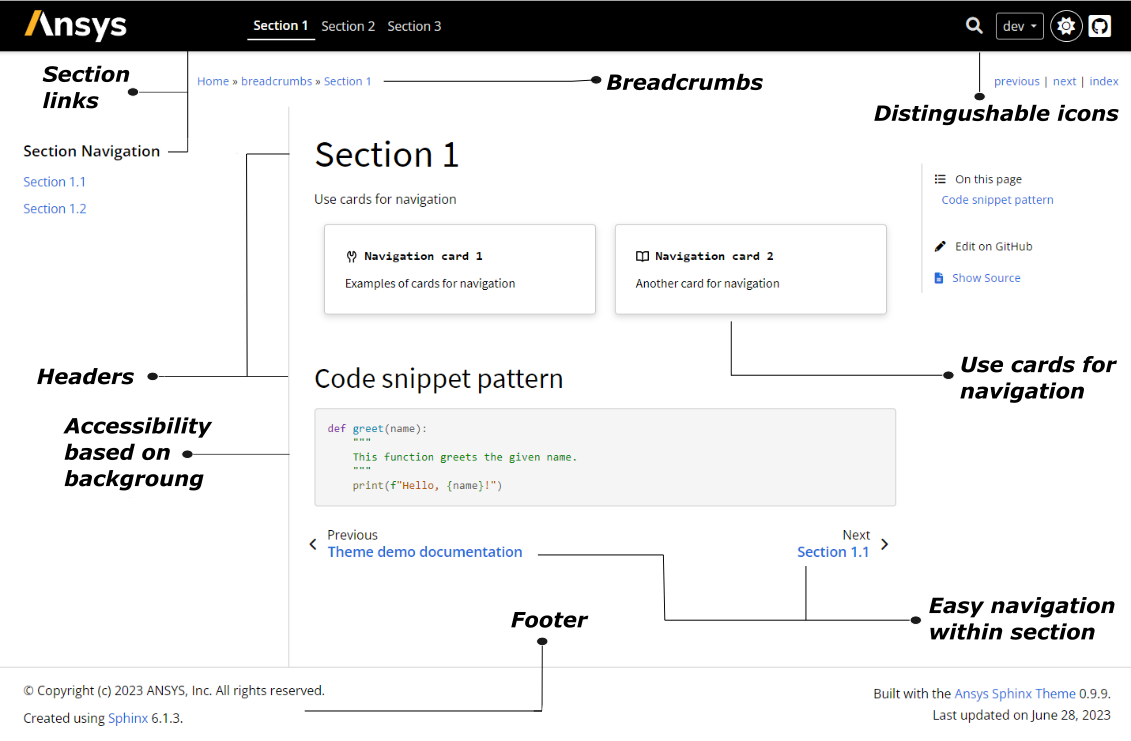
\includegraphics[width=\textwidth]{img/documentation/docs-example}
\vspace{-14cm}
}{
%%%% Bottom space

%% QR code

\qrcode{img/documentation/qrcode.png}{img/general/smartphoneBlack}{
\textbf{Want to see our documentation theme site?} \\ \checkmark Visit https:\slash \slash sphinxdocs.ansys.com for more information \\ \newline \textbf{Any doubts?} \\ \checkmark Don't be shy and start the conversation!
}
% Smartphone icon
% Author: Freepik
% Retrieved from: https://www.flaticon.com/free-icon/smartphone_65680

%% Compact QR code (comment the previous command and uncomment this one to switch)
%\compactqrcode{img/example/qrcode}{
%\textbf{Take a picture} to
%\\download the full paper
%}

}

}{
%%%%%%%% LEFT COLUMN


\title{Accessible \\documentation \\for everyone}
\author{Revathy Venugopal}
\institution{Ansys}

\section{
\includegraphics[height=\fontcharht\font`\S]{img/general/slash.png} Introduction}
Accessible documentation emphasizes inclusive document creation for universal understanding. 
Uncover practical strategies to foster equitable information access, empowering you to produce 
improved, accessible documents for all.

\section{
\includegraphics[height=\fontcharht\font`\S]{img/general/slash.png} Accessibility guidelines}

\begin{itemize}
\item Readable fonts
\item Structured document with headings
\item Alternative text (Alt Text) for images
\item Color contrast considerations
\item Multimedia accessibility
\item Accessible document formats
\end{itemize}

\section{
\includegraphics[height=\fontcharht\font`\S]{img/general/slash.png} Document navigation}

\begin{itemize}
\item Use clear and consistent navigation elements
\item Skip navigation links to bypass redundant content
\item Implement breadcrumb navigation
\item Include a search function
\item Ensure keyboard accessibility
\end{itemize}

}{
%%%%%%%% RIGHT COLUMN

\section{
\includegraphics[height=\fontcharht\font`\S]{img/general/slash.png} Inclusive visual design}

\begin{itemize}
\item Clear and distinguishable icons and graphic
\item Use accessible color palettes
\item Consider font choices
\item Optimize design for different screen sizes and resolutions
\item Prioritize adequate white space
\end{itemize}

\section{
\includegraphics[height=\fontcharht\font`\S]{img/general/slash.png} Document versioning}

\begin{itemize}
\item Ensure backward compatibility
\item Provide clear documentation of accessibility considerations and changes in each version.
\item Seek feedback from users
\end{itemize}

\section{
\includegraphics[height=\fontcharht\font`\S]{img/general/slash.png} Conclusion}

Making our documentation as accessible as possible to the widest audience we can, helps all our readers engage with the content.

\vfill


\includegraphics[width=\textwidth]{img/general/pyansys_dark}\\
The PyAnsys project is a collection of Python packages that enable the use of Ansys products through Python.
\\
\newline
\textbf{Any doubts?} \\Contact us at pyansys.core@ansys.com!
\\
\newline

\qrcode{img/general/pyansys_qrcode.png}{img/general/smartphoneBlack}{
\textbf{\huge{Check our docs for more\\information on PyAnsys!\\https:\slash \slash docs.pyansys.com }}
}
}
\end{document}
